\hypertarget{progettazione}{%
\chapter{Progettazione}\label{progettazione}}

\hypertarget{architettura-del-sistema}{%
\section{Architettura del sistema}\label{architettura-del-sistema}}

L'architettura utilizzata da GeneroCity è del tipo \emph{client-server}.

\begin{figure}[H]
\centering
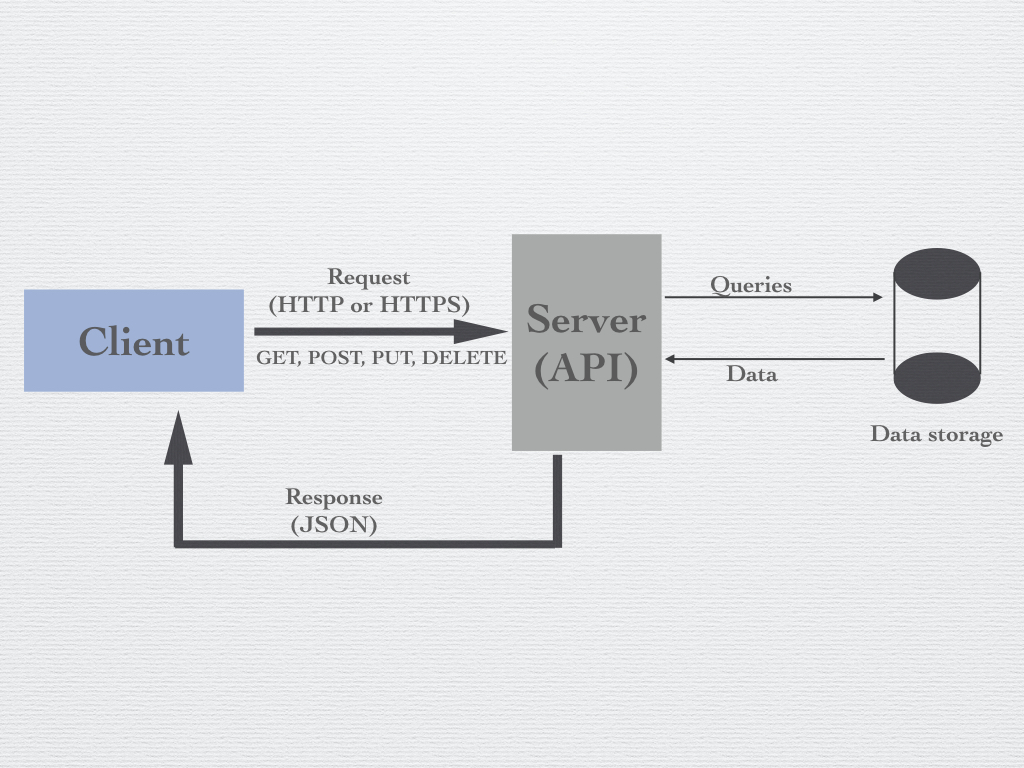
\includegraphics[width=12cm]{rest_architecture.jpg}
\caption{Diagramma di un'architettura client-server con API REST \cite{what-is-restful-api}}
\end{figure}


Il \emph{client}, ovvero il dispositivo Android dell'utente, comunica con il \emph{server} mediante delle chiamate alle API REST. La comunicazione permette al client l'accesso a delle risorse, ovvero a delle informazioni che il server decide di rendere disponibili per il client. \cite{rest-api-design}

La comunicazione avviene tramite il protocollo HTTP.

Una chiamata alle API REST contiene i seguenti elementi:

\begin{itemize}
    \item \textbf{\emph{Uniform Resource Identifier}} (\emph{URI}): indirizzo che indica dove trovare la risorsa su Internet;
    \item \textbf{Metodo} \texttt{HTTP}: indica l'operazione che bisogna effettuare con la risorsa indicata dall'URI. I principali metodi sono quattro:

 \begin{itemize}     \item  \texttt{GET}: permette di recuperare la risorsa, la quale verrà  mostrata in uno specifico formato (solitamente XML o JSON);     \item  \texttt{POST}: sostituisce la risorsa con un'altra risorsa,  solitamente indicata nel body;     \item  \texttt{PUT}: crea una nuova risorsa;     \item  \texttt{DELETE}: elimina la risorsa indicata. \end{itemize}
    \item \texttt{Header}: è una parte del messaggio che contiene delle informazioni chiave per entrambi il server ed il client. Tali informazioni possono essere ad esempio il formato della risposta, la chiave dell'API o l'indirizzo IP del server.
    \item \texttt{Body} (opzionale): viene utilizzato per inviare o ricevere ulteriori parti di dati.
\end{itemize}

\hypertarget{progettazione-ed-implementazione-di-funzionalituxe0-minori}{%
\section{Funzionalità minori}\label{progettazione-ed-implementazione-di-funzionalituxe0-minori}}

\hypertarget{implementazione-della-lista-dei-parcheggi}{%
\subsection{Implementazione della lista dei parcheggi}\label{implementazione-della-lista-dei-parcheggi}}

Lo scopo dell'implementazione dell'interfaccia di cui si andrà a parlare è quello di mostrare agli utenti uno storico dei parcheggi che sono stati effettuati.

Tali parcheggi vengono inseriti all'interno di una lista, implementata in Android mediante una \texttt{RecyclerView}, i cui i singoli elementi sono cliccabili.

Il click su un elemento che modella un singolo parcheggio porta ad una schermata contenente maggiori dettagli su tale parcheggio.

\begin{figure}[H]
\centering
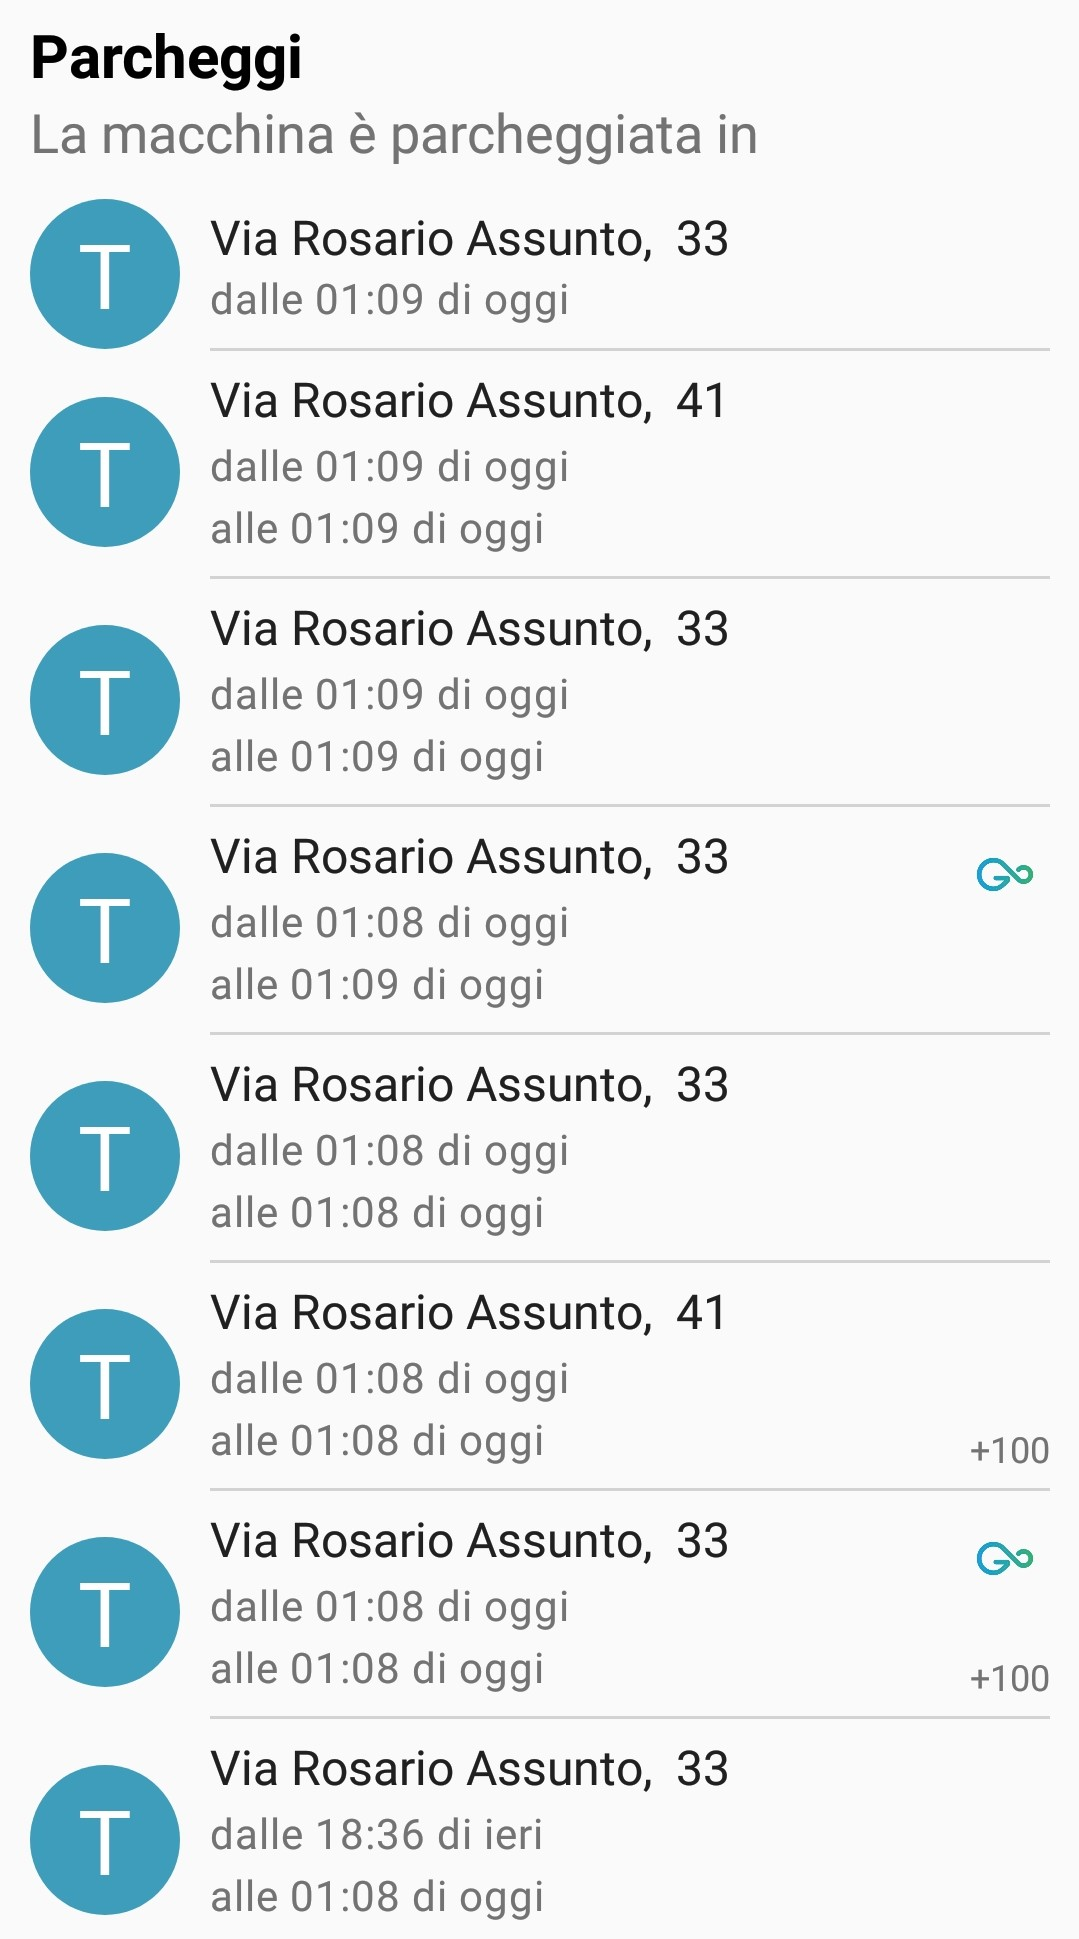
\includegraphics[width=6cm]{storico_parcheggi.jpg}
\caption{Storico parcheggi}
\label{storico-parcheggi}
\end{figure}

Negli elementi che compongono la lista sono presenti tre dati:

\begin{itemize}
    \item L'indirizzo, composto da via e civico, dove la macchina è stata parcheggiata
    \item L'orario e la data in cui la macchina è stata parcheggiata
    \item L'orario e la data in cui l'utente è uscito dal parcheggio
\end{itemize}
Il primo elemento della lista modella il parcheggio in cui l'auto dell'utente è correntemente situata. Essendo il parcheggio ancora in corso, non viene mostrato l'orario e la data in cui l'utente lo ha terminato. 

L'implementazione della lista dei parcheggi è stata sviluppata insieme ad altri due membri del team di sviluppo, a differenza delle altre funzioni di cui si parlerà nel resto della relazione.

\subsubsection{Paginazione dei risultati}

Prima dell'implementazione della funzionalità che verrà descritta, lo storico mostrava solamente gli ultimi 16 parcheggi effettuati dall'utente.

Questo avviene in quanto la chiamata alle API per ottenere la lista dei parcheggi effettuati con una macchina (\texttt{/car/\{cid\}/park/}) richiede opzionalmente come \emph{query parameter} un id del parcheggio.

Se questo parametro non viene inserito, l'API restituisce la lista degli ultimi 16 parcheggio effettuati, altrimenti restituisce la lista dei 16 parcheggi effettuati precedentemente al parcheggio passato come parametro.

Tramite questa logica è stato possibile paginare lo storico del parcheggi.

L'utente quando apre la schermata visualizza solo i 16 parcheggi più recenti. Quando effettua uno \emph{scroll} ed arriva in fondo alla pagina, l'app effettua una chiamata alle API inserendo come parametro l'ultimo parcheggio della lista, in maniera da recuperare i 16 parcheggi antecedenti all'ultimo parcheggio mostrato.

Durante la richiesta viene mostrata una progress bar, che viene rimossa quando i risultati sono disponibili.

Una volta che ciò accade, vengono inseriti ulteriori 16 parcheggi, o meno se i parcheggi totali sono inferiori, all'interno dello storico.

L'utente può continuare ad effettuare uno \emph{scroll} finché non visualizza tutti i parcheggi effettuati dalla macchina corrente.

\hypertarget{indicatori-di-scambio-nel-parcheggio}{%
\subsection{Indicatori di scambio nel parcheggio}\label{indicatori-di-scambio-nel-parcheggio}}

\begin{figure}[H]
\centering

\includegraphics[width=3cm]{images/gc-logo.png}
\caption{Logo di GeneroCity.}
\label{gc-logo}
\end{figure}

Aprendo lo storico dei parcheggi effettuati dall'utente, non era possibile capire a colpo d'occhio quali fossero i parcheggi effettuati tramite uno scambio con un altro utente, e quali fossero quelli effettuati senza uno scambio

Per ovviare a questa problematica, sono state inserite due icone alla destra di ogni elemento della lista dello storico dei parcheggi, che fanno capire all'utente la natura dello scambio (se presente). È possibile vedere una rappresentazione delle icone nella \autoref{storico-parcheggi}

L'icona presente in \autoref{gc-logo} è presente se il parcheggio è stato ottenuto mediante il completamento di un match; mentre il testo che indica "+100" è presente se il parcheggio è stato lasciato ad un utente mediante il completamento di un match. 

\pagebreak


\hypertarget{progettazione-del-sistema-di-scambio}{%
\section{Gestione dei matches}\label{progettazione-del-sistema-di-scambio}}

Nella seguente sezione verranno mostrate e documentate le interfacce che sono state realizzate ed il processo che ha portato alla loro realizzazione.

In particolare, sono state realizzate le schermate che permettono all'utente di:
\begin{itemize}      \item Comunicare al sistema l'intenzione di lasciare il posto ad un altro utente (diventare giver);      \item Chiedere al sistema di trovare un posto disponibile da occupare (diventare Taker);      \item Permettere di vedere se il sistema stia attualmente cercando un utente con ruolo opposto compatibile con cui scambiare il posto, ed eventualmente annullare tale ricerca;      \item Permettere di vedere informazioni utili circa il match in corso, come  la posizione del Taker e del Giver, il percorso tra il  Taker ed il Giver ed il tempo stimato di arrivo.
\end{itemize}
\hypertarget{cosuxe8-un-match}{%
\paragraph{Cos'è un match}\label{cosuxe8-un-match}}

Quando un utente parcheggiato comunica all'app di voler lasciare il posto, egli diventa un Giver.

Quando invece un utente comunica all'app di voler cercare un posto disponibile da occupare, diventa un Taker.

Quando un Taker ed un Giver sono compatibili, viene effettuato un \emph{match}. Quando si è all'interno di un match in corso, il Giver attende l'arrivo del Taker. Quando il
Taker raggiunge il Giver, quest'ultimo può lasciare il posto, che verrà occupato dal Taker. In tal caso il match viene completato con successo.

Il Taker ha un tempo di 15 minuti per raggiungere il Giver prima che il match venga annullato.

\hypertarget{struttura-delle-schermate}{%
\subsection{Struttura delle schermate}\label{struttura-delle-schermate}}

Le schermate che sono state progettate hanno tutte la medesima struttura, rappresentata nella \autoref{wireframe}.

\begin{figure}[H]
\centering
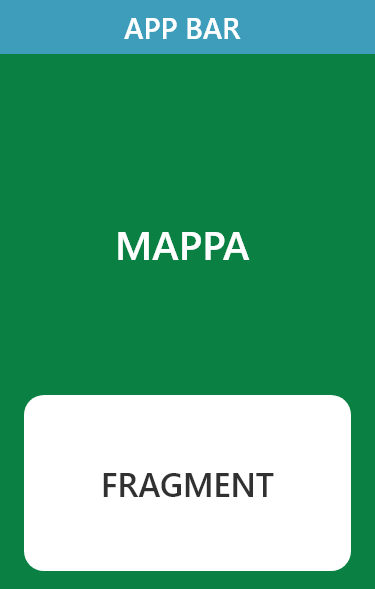
\includegraphics[width=6cm]{images/wireframe.png}
\caption{Wireframe delle schermate implementate.}
\label{wireframe}
\end{figure}

In alto è presente l'app bar, la quale contiene il nome dell'applicazione e dei pulsanti per effettuare delle azioni contestuali alla schermata in cui l'utente si trova.

Sottostante all'app bar è presente la mappa, ovvero un \texttt{Fragment} contenente una mappa fornita da Google su cui è possibile mostrare degli elementi.

Nella parte inferiore dello schermo è presente un \texttt{Fragment} che verrà sostituito a seconda della natura della schermata.

Il \texttt{Fragment} che viene mostrato all'apertura dell'applicazione è il \texttt{CarFragment} , già esistente all'inizio del tirocinio.

I metodi per effettuare le operazioni sui \texttt{Fragments} sono inseriti all'interno di una classe \texttt{FragmentUtility}.

Nei paragrafi successivi si parlerà proprio dei vari \texttt{Fragments} che sono stati sviluppati, e del modo in cui sono stati integrati all'interno del resto dell'interfaccia.

\hypertarget{toggle-per-registrare-e-rimuovere-un-parcheggio}{%
\subsection{Registrare e rimuovere un parcheggio}\label{toggle-per-registrare-e-rimuovere-un-parcheggio}}

L'applicazione registra un parcheggio quando una delle due condizioni si verifica:

\begin{itemize}
    \item L'utente preme il pulsante \texttt{PARCHEGGIATA} nella schermata principale;
    \item L'utente è in stato di \texttt{DidExitCar}.
\end{itemize}
L'applicazione rimuove un parcheggio quando una delle due condizioni si verifica:

\begin{itemize}
    \item L'utente preme il pulsante \texttt{IN USO} nella schermata principale;
    \item L'utente è in stato di \texttt{DidEnterCar}.
\end{itemize}
Il bottone per parcheggiare e rimuovere il parcheggio manualmente viene inserito in quanto il sistema potrebbe errare nella rilevazione automatica dello stato dell'utente (parcheggiato o non parcheggiato), e quindi all'utente viene data la possibilità di riallineare il sistema alla realtà, comunicando lo stato della macchina come ``parcheggiata'' o ``in uso'' mediante dei pulsanti dedicati.

\begin{figure}[H]
\centering
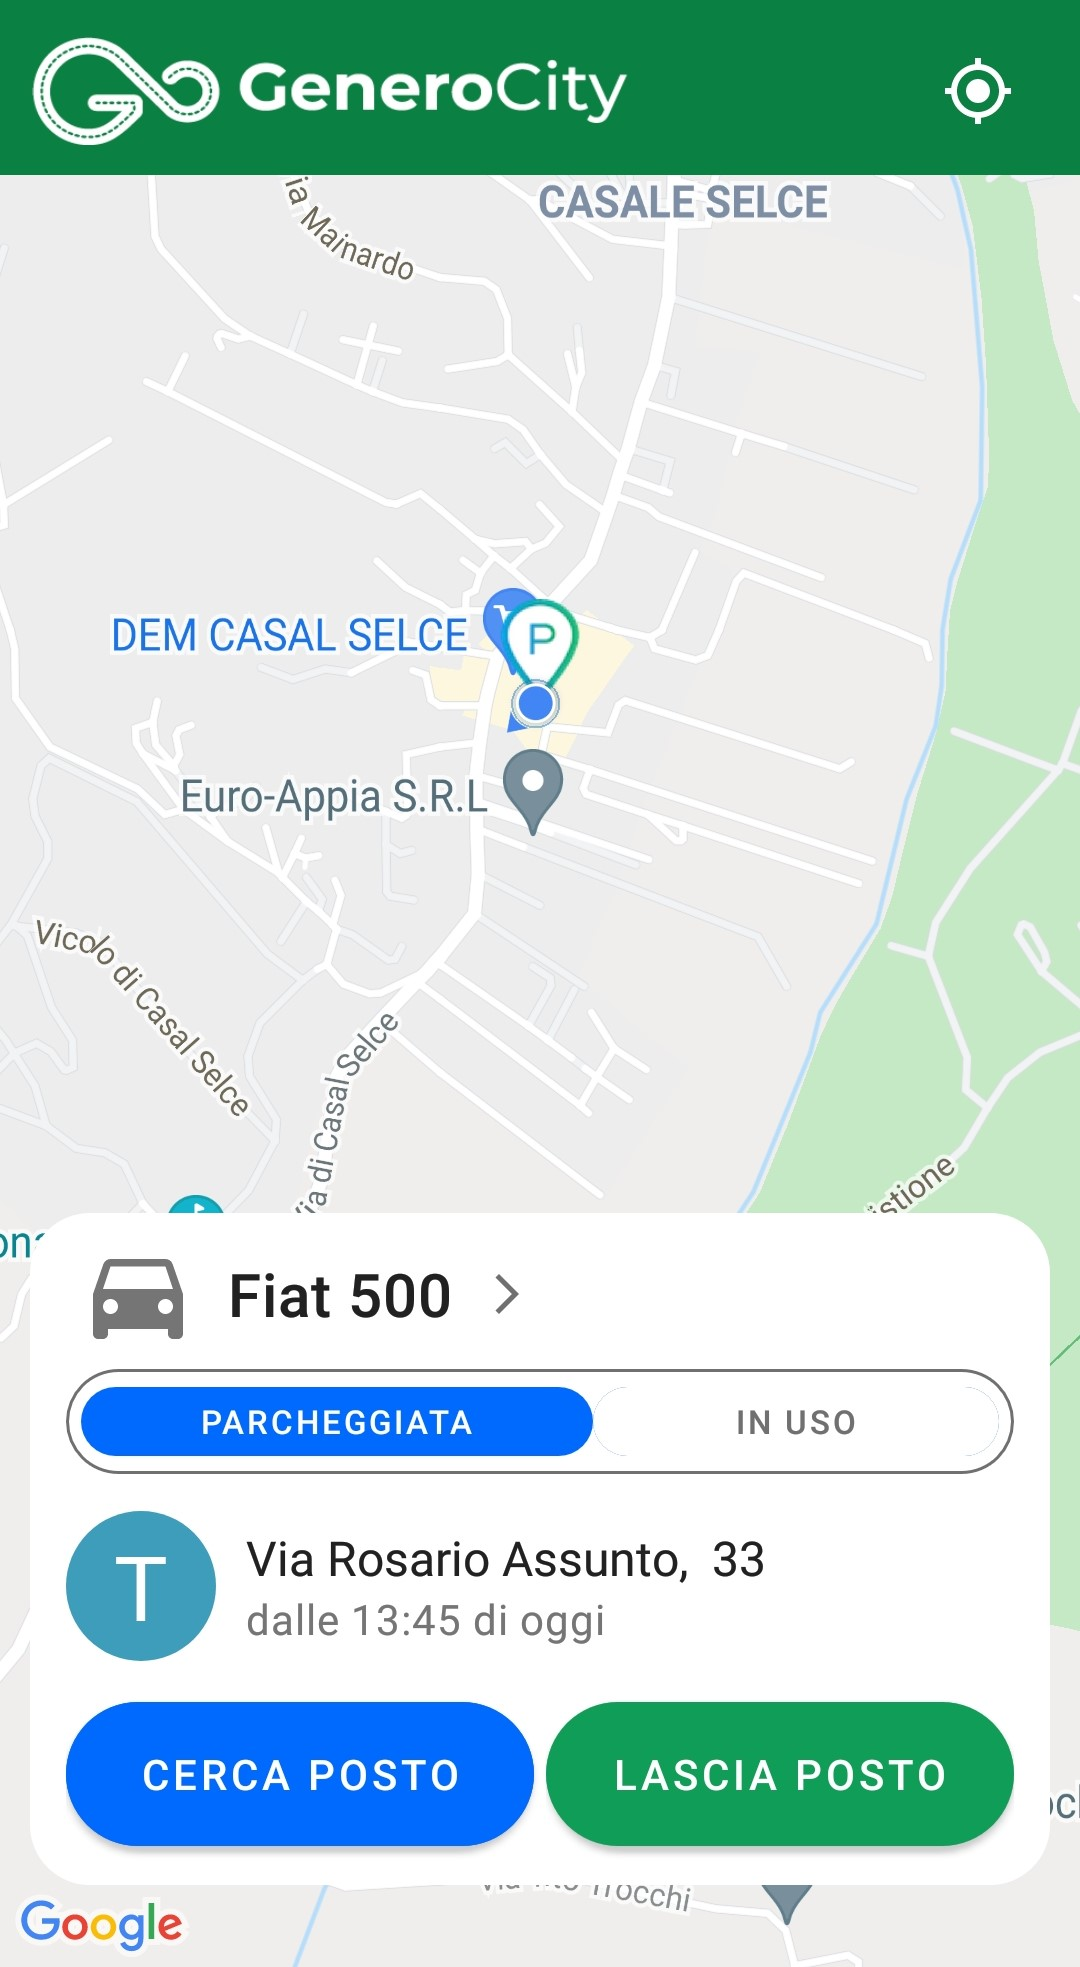
\includegraphics[width=6cm]{park_button_parked.jpg}
\caption{Interfaccia della pagina principale quando l'auto è parcheggiata.}
\end{figure}

In questo caso l'auto è parcheggiata e l'utente può premere sul pulsante \texttt{IN USO} per rimuovere tale parcheggio e comunicare all'applicazione che l'auto è attualmente in uso.

\begin{figure}[H]
\centering
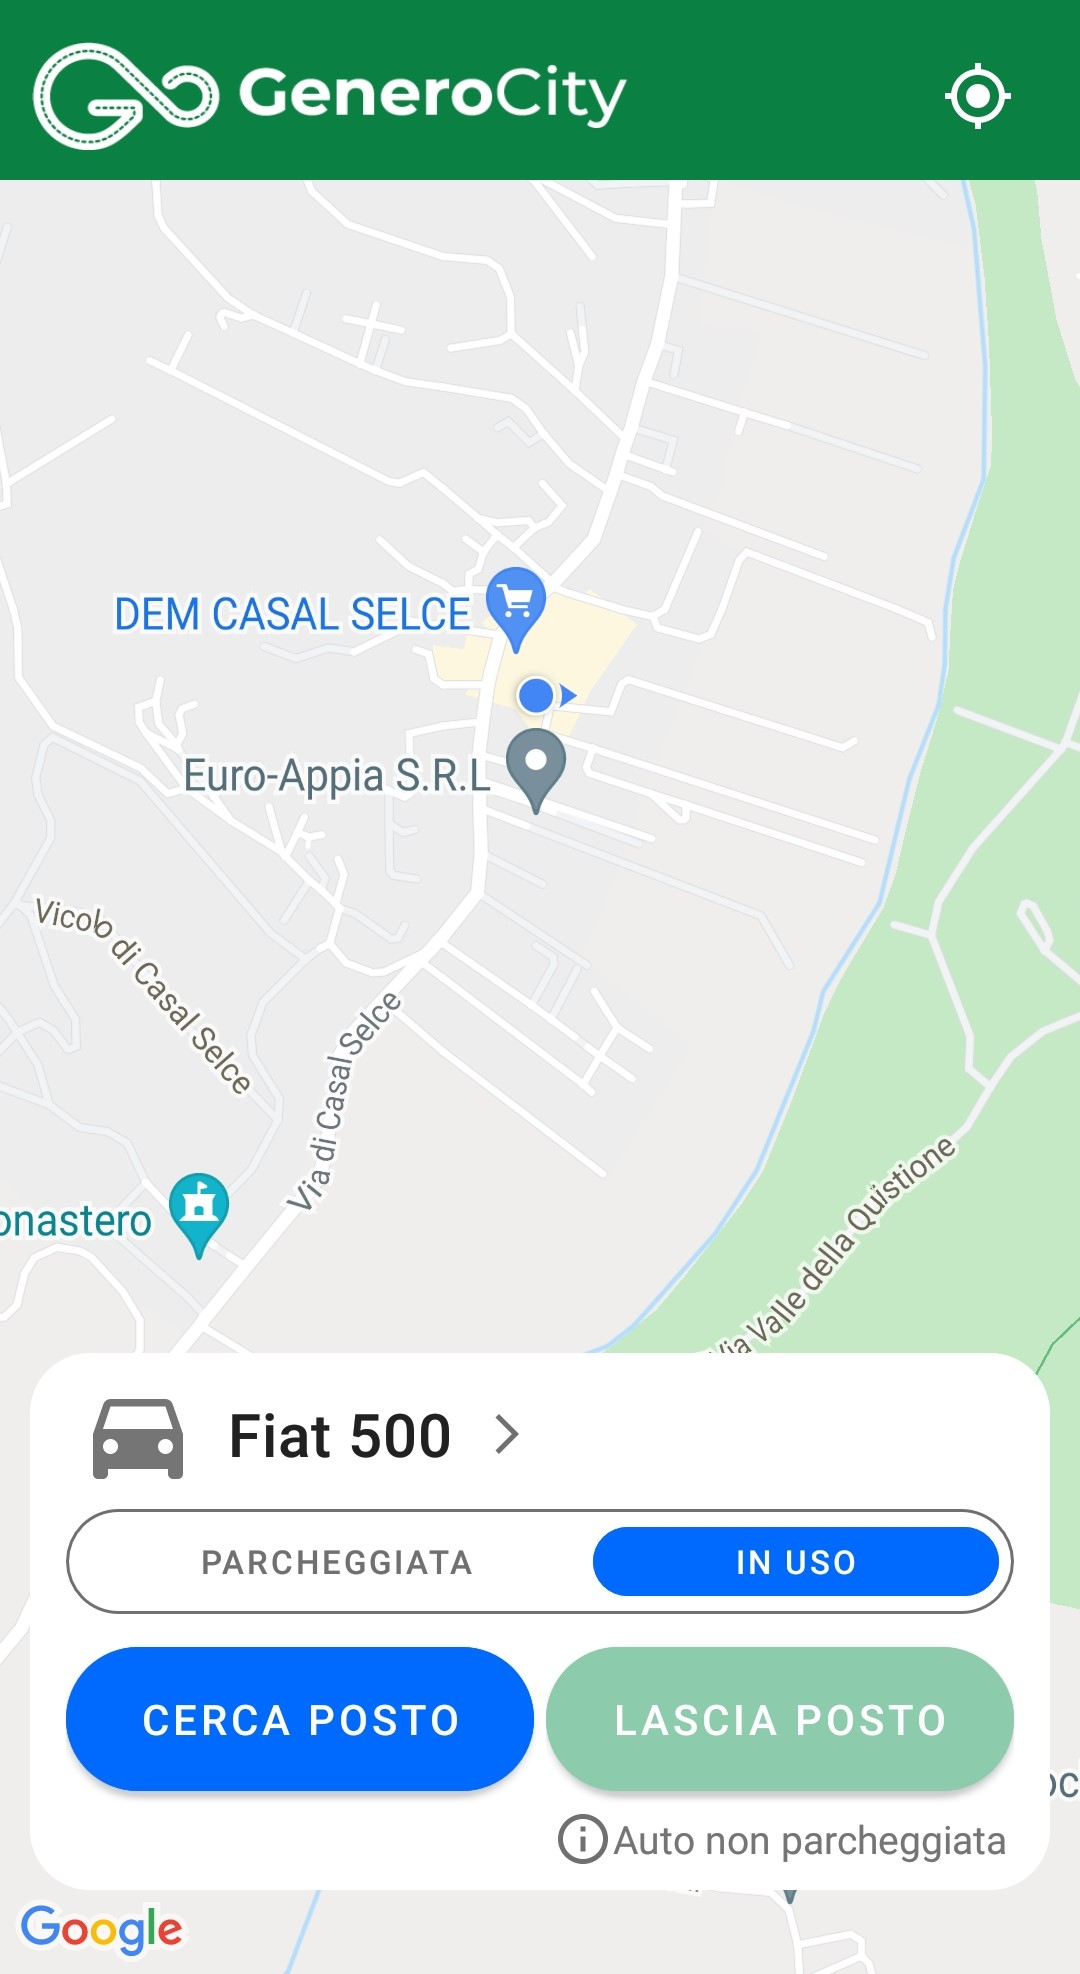
\includegraphics[width=6cm]{park_button_use.jpg}
\caption{Interfaccia della pagina principale quando l'auto è in uso.}
\end{figure}

In questo caso l'auto è in uso, ma l'utente può premere il pulsante \texttt{PARCHEGGIATA} per parcheggiare l'auto nella sua posizione attuale.

\hypertarget{test-effettuati}{%
\subsubsection{Test effettuati}\label{test-effettuati}}

Per verificare se ci fossero dei problemi legati all'usabilità dell'interfaccia, sono stati effettuati dei test sul campo con degli utenti.

Tali utenti sono stati inseriti in un'ipotetica situazione in cui il sistema segnalava che la loro macchina fosse in uso, quando in realtà questa era parcheggiata. Si è quindi chiesto loro di comunicare al sistema il fatto che l'auto fosse parcheggiata nel luogo in cui ora loro si trovavano.

Agli stessi utenti è stato effettuato anche il test inverso, e quindi è stato detto loro di comunicare al sistema che la macchina non era realmente parcheggiata in un luogo, ma che fosse attualmente in uso.

Tutti i test sono andati a buon fine e quindi si è concluso che l'interfaccia fosse utilizzabile in maniera corretta.

\hypertarget{interfaccia-per-ricerca-di-un-match}{%
\subsection{Ricerca di un match}\label{interfaccia-per-ricerca-di-un-match}}

La classe \texttt{FindMatchFragment} modella un \texttt{Fragment} che viene mostrato all'utente quando è in corso una ricerca, da parte del sistema, di un utente compatibile con cui effettuare uno scambio.

Si accede a tale schermata in tre modi:

\begin{itemize}
    \item Premendo il bottone ``cerca posto'' nella schermata inziale.
    \item Premendo il bottone ``lascia posto'' nella schermata iniziale.
    \item In caso di ripristino dello stato dell'\emph{activity} dopo che questa è stata chiusa.
\end{itemize}
Il \texttt{FindMatchFragment} rimpiazza sempre il \texttt{CarFragment}.

Per evitare duplicazione di codice, il \texttt{Fragment} utilizza solo un layout \texttt{xml} il quale viene modificato a tempo di esecuzione a seconda del ruolo dell'utente, in maniera da mostrare le informazioni utili al Taker o al giver.

La \emph{\texttt{view}} del \texttt{fragment} mostra all'utente i seguenti elementi:

\begin{itemize}
    \item Una \emph{label}, differente da Taker a Giver, che indica cosa l'utente stia cercando;
    \item Una \emph{progress bar} circolare che mostra all'utente che il processo di ricerca è in corso;
    \item Un bottone per annullare la ricerca.
\end{itemize}

\begin{figure}[H]
\centering
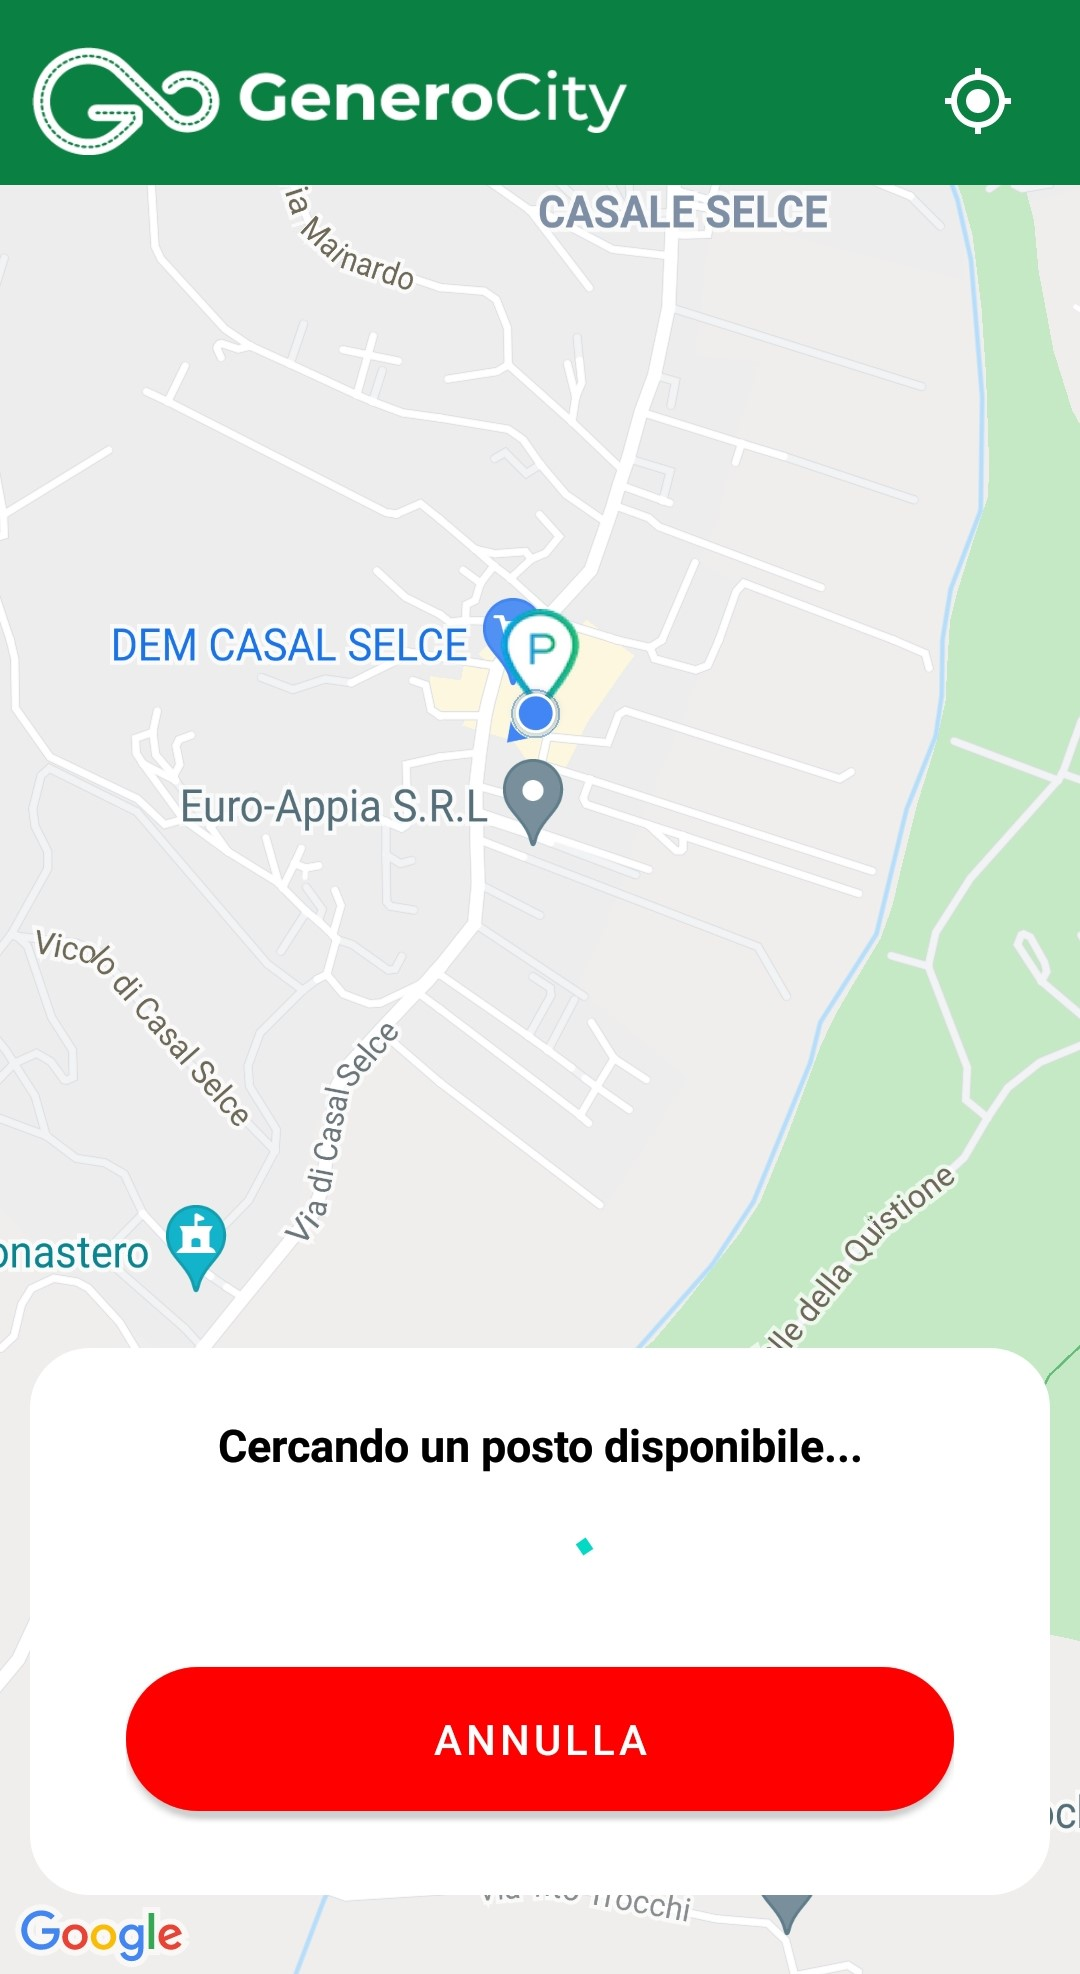
\includegraphics[width=6cm]{images/find_giver.jpg}
\caption{Interfaccia mostrata durante la ricerca di un Giver.}
\end{figure}

In caso del Taker, la label mostra la scritta ``Cercando un posto disponibile''


\begin{figure}[H]
\centering
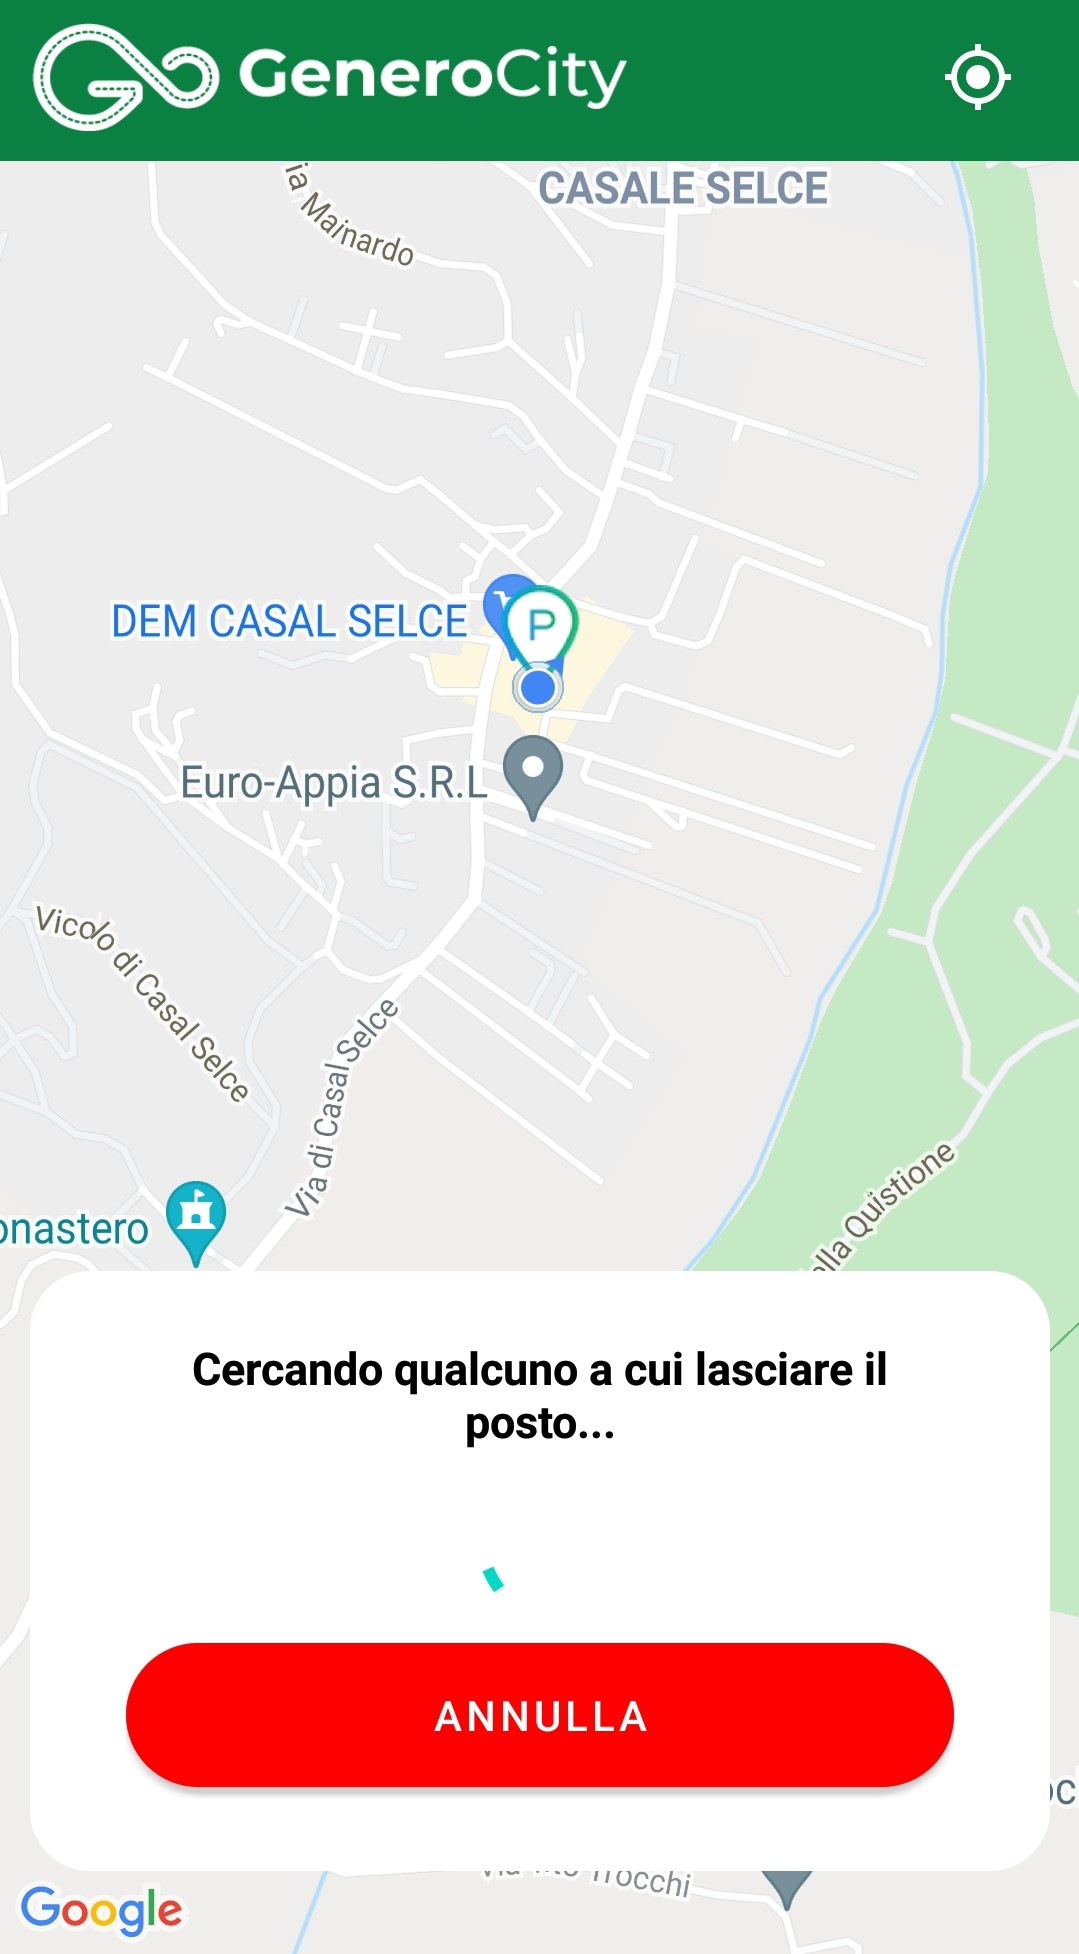
\includegraphics[width=6cm]{find_taker.jpg}
\caption{Interfaccia mostrata durante la ricerca di un Taker.}
\end{figure}

In caso del Giver, la label mostra la scritta ``Cercando qualcuno a cui lasciare il posto''.

\hypertarget{interfaccia-per-match-effettuato}{%
\subsection{Match effettuato}\label{interfaccia-per-match-effettuato}}

La classe \texttt{MatchFoundFragment} modella un \texttt{Fragment} che viene mostrato all'utente quando il sistema ha trovato un utente compatibile con cui effettuare uno scambio, e tale scambio è in corso di esecuzione.

La schermata può essere raggiunta dall'utente in tre modi:

\begin{itemize}
    \item Quando il sistema, per un utente nel ruolo di Taker, trova un utente Giver compatibile;
    \item Quando il sistema, per un utente nel ruolo di Giver, trova un utente Taker compatibile;
    \item In caso di ripristino dello stato dell'\emph{activity} dopo che questa è stata chiusa.
\end{itemize}
Nei primi due casi il \texttt{MatchFoundFragment} rimpiazza il
\texttt{FindMatchFragment}.

Nel terzo caso la UI si trova nella schermata iniziale, dove il Fragment mostrato sotto la mappa è il \texttt{CarFragment}. Per questo, quando la UI verrà ripristinata, il \texttt{MatchFoundFragment} ripristina il
\texttt{CarFragment}.

Anche qui è stato utilizzato un solo layout \texttt{xml} per evitare duplicazione di codice.


\begin{figure}[H]
\centering
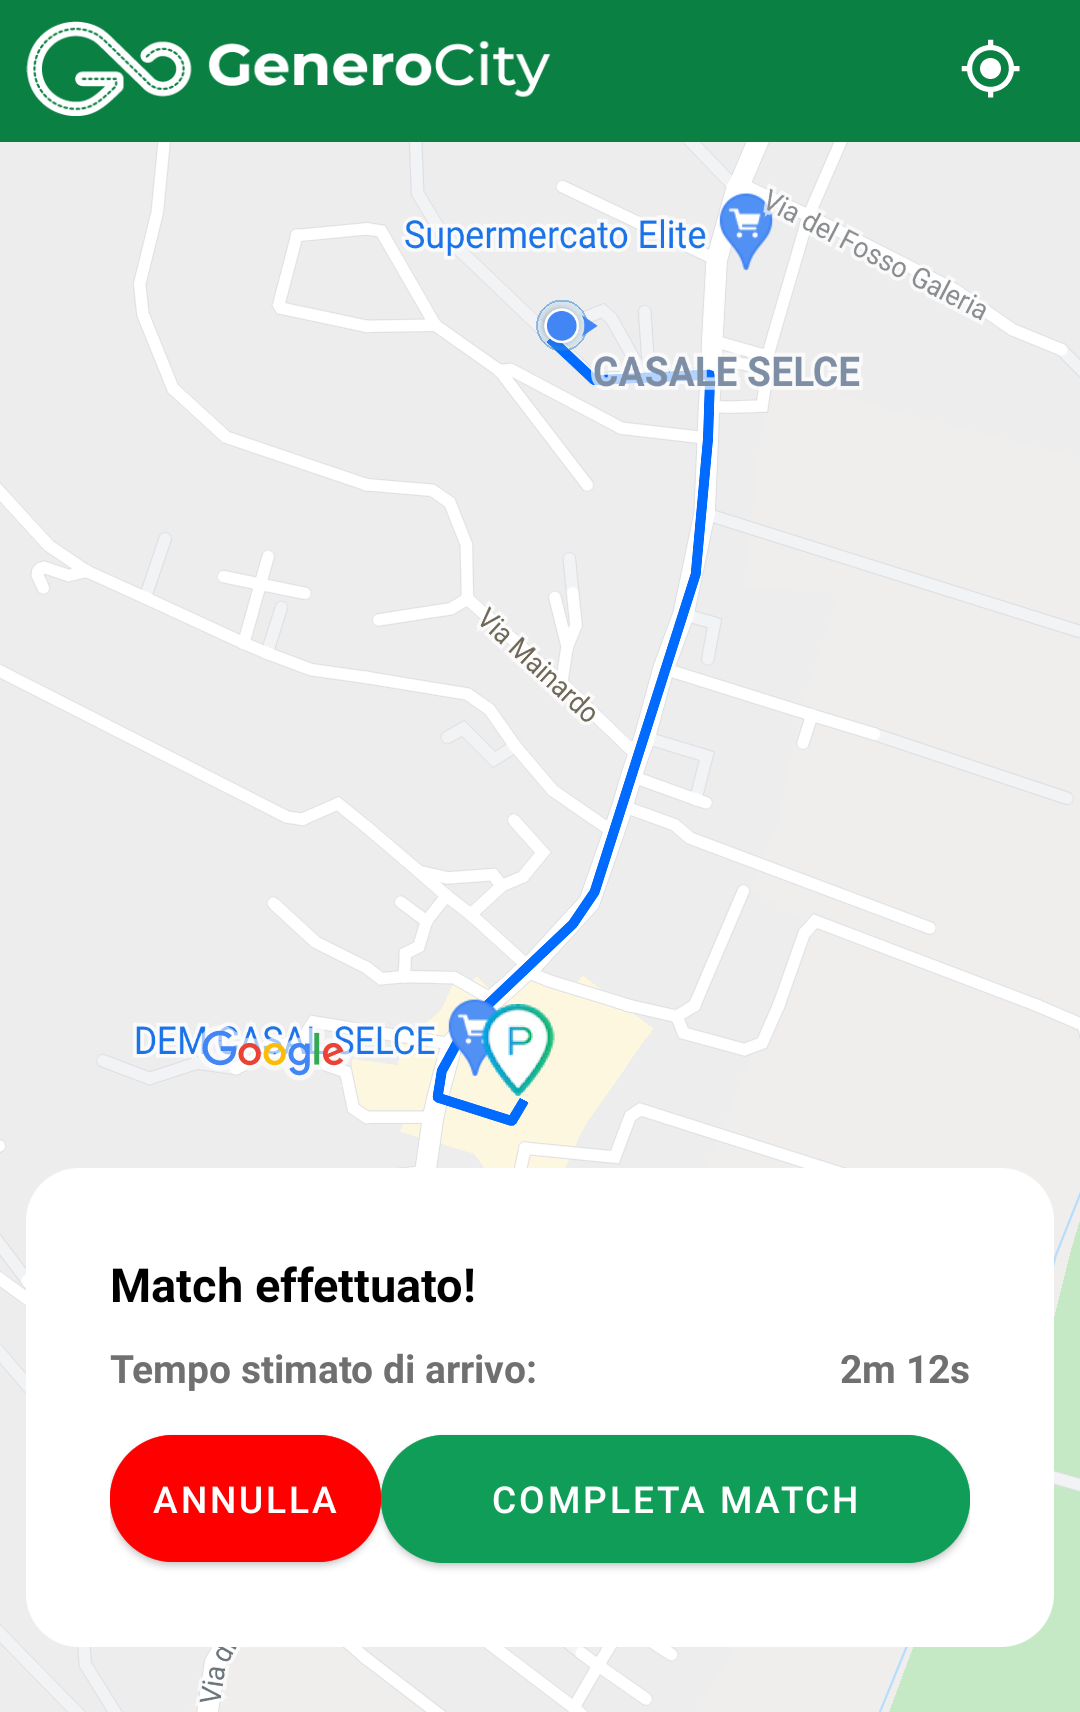
\includegraphics[width=6cm]{match_found_taker.png}
\caption{Interfaccia mostrata al Taker quando ha trovato un
Giver compatibile.}
\label{match-found-taker}
\end{figure}

Nel \texttt{Fragment} mostrato al Taker sono presenti quattro elementi:

\begin{itemize}
    \item Una \emph{label} che indica che un match è stato effettuato, e quindi che è presente un Giver compatibile pronto a cedere il posto auto;
    \item Una \emph{label} che indica il tempo stimato circa l'incontro tra i due utenti;
    \item Un bottone con dicitura ``Annulla'' che permette di annullare il match in corso. Sia il Taker che il Giver verranno portati nella pagina principale dell'applicazione;
    \item Un bottone con dicitura ``Completa match'' che permette di segnalare il match come confermato. Sia il Taker che il Giver verranno portati nella pagina principale dell'applicazione;
\end{itemize}
Nella mappa sono presenti tre elementi:

\begin{itemize}
    \item L'icona che rappresenta il punto in cui è parcheggiato il \emph{giver,} ovvero il punto che il Taker dovrà raggiungere;
    \item L'icona che rappresenta la posizione aggiornata del Taker, ovvero dell'utente che visualizza tale schermata;
    \item Il percorso che il Taker deve effettuare per arrivare dal giver;
\end{itemize}
\hypertarget{percorso-per-arrivare-dal-giver}{%
\subsubsection{Percorso per arrivare dal giver}\label{percorso-per-arrivare-dal-giver}}

Il percorso mostrato sulla mappa, che indica la strada che il Taker deve percorrere per arrivare dal Giver mediante un'automobile, è stato ottenuto mediante le \emph{Google Directions API}.

Il Taker, quando trova un Giver compatibile, effettua una chiamata alle Directions API all'url
\begin{verbatim}
    https://maps.googleapis.com/maps/api/directions/json
\end{verbatim}
in cui vengono inseriti come \textit{query parameters}, i seguenti campi:
\begin{itemize}
    \item \texttt{origin}: le coordinate (o indirizzo) del punto d'origine, ovvero l'attuale posizione del Taker;
    \item \texttt{destination}: le coordinate (o indirizzo) del punto destinazione, ovvero la posizione del Giver;
    \item \texttt{key}: la chiave per poter utilizzare le API.
\end{itemize}

Tale chiamata ritorna un oggetto json in cui sarà presente, in aggiunta ad altre informazioni, una codifica delle \texttt{Polylines} da inserire sulla mappa per mostrare il percorso tra i due punti.

Una \texttt{Polyline} è un segmento che mostra sulla mappa il collegamento tra due punti. La serie di \texttt{Polylines} che deve essere mostrata viene codificata da un algoritmo.
\begin{lstlisting}[caption=Lista di \texttt{Polylines} codificata]
    kox~Fq_kjALDGb@_@E]MMG]]qAuBq@eAY_@OOe@SqC}@yC}@gC}@o@KcGQqCIc@Ia
    A]aGsC}E{BeBw@oAg@UCQYg@c@c@g@[g@ESAwA@aA?kCLsCHiAFQ[k@W_@W_@c@}@
    _@aAs@eCWeBMe@GMaBgBeC}Be@]{A{@}@s@i@UiDeAeAO]Oc@WN{CJw@Z}@Ve@pAc
    BJ[Da@AoBHm@d@}Ab@}@lAmBb@m@SQMAe@Fs@Ca@?y@R}@f@yAlA[NqBh@sB`AQ@W
    ID_@@SFSFI\\OLQHg@?UG[u@wAO]UkAQg@]c@o@k@oBkAq@e@SWk@}@{@{BMw@PoF
    BgA?{@Es@CYG]u@G
\end{lstlisting}
 Il messaggio viene decodificato in un vettore di oggetti \texttt{LatLng}, che verranno utilizzati per costruire le varie \texttt{Polylines} sulla mappa, che nell'insieme formeranno il percorso mostrato in \autoref{match-found-taker}. 

\begin{figure}[H]
\centering
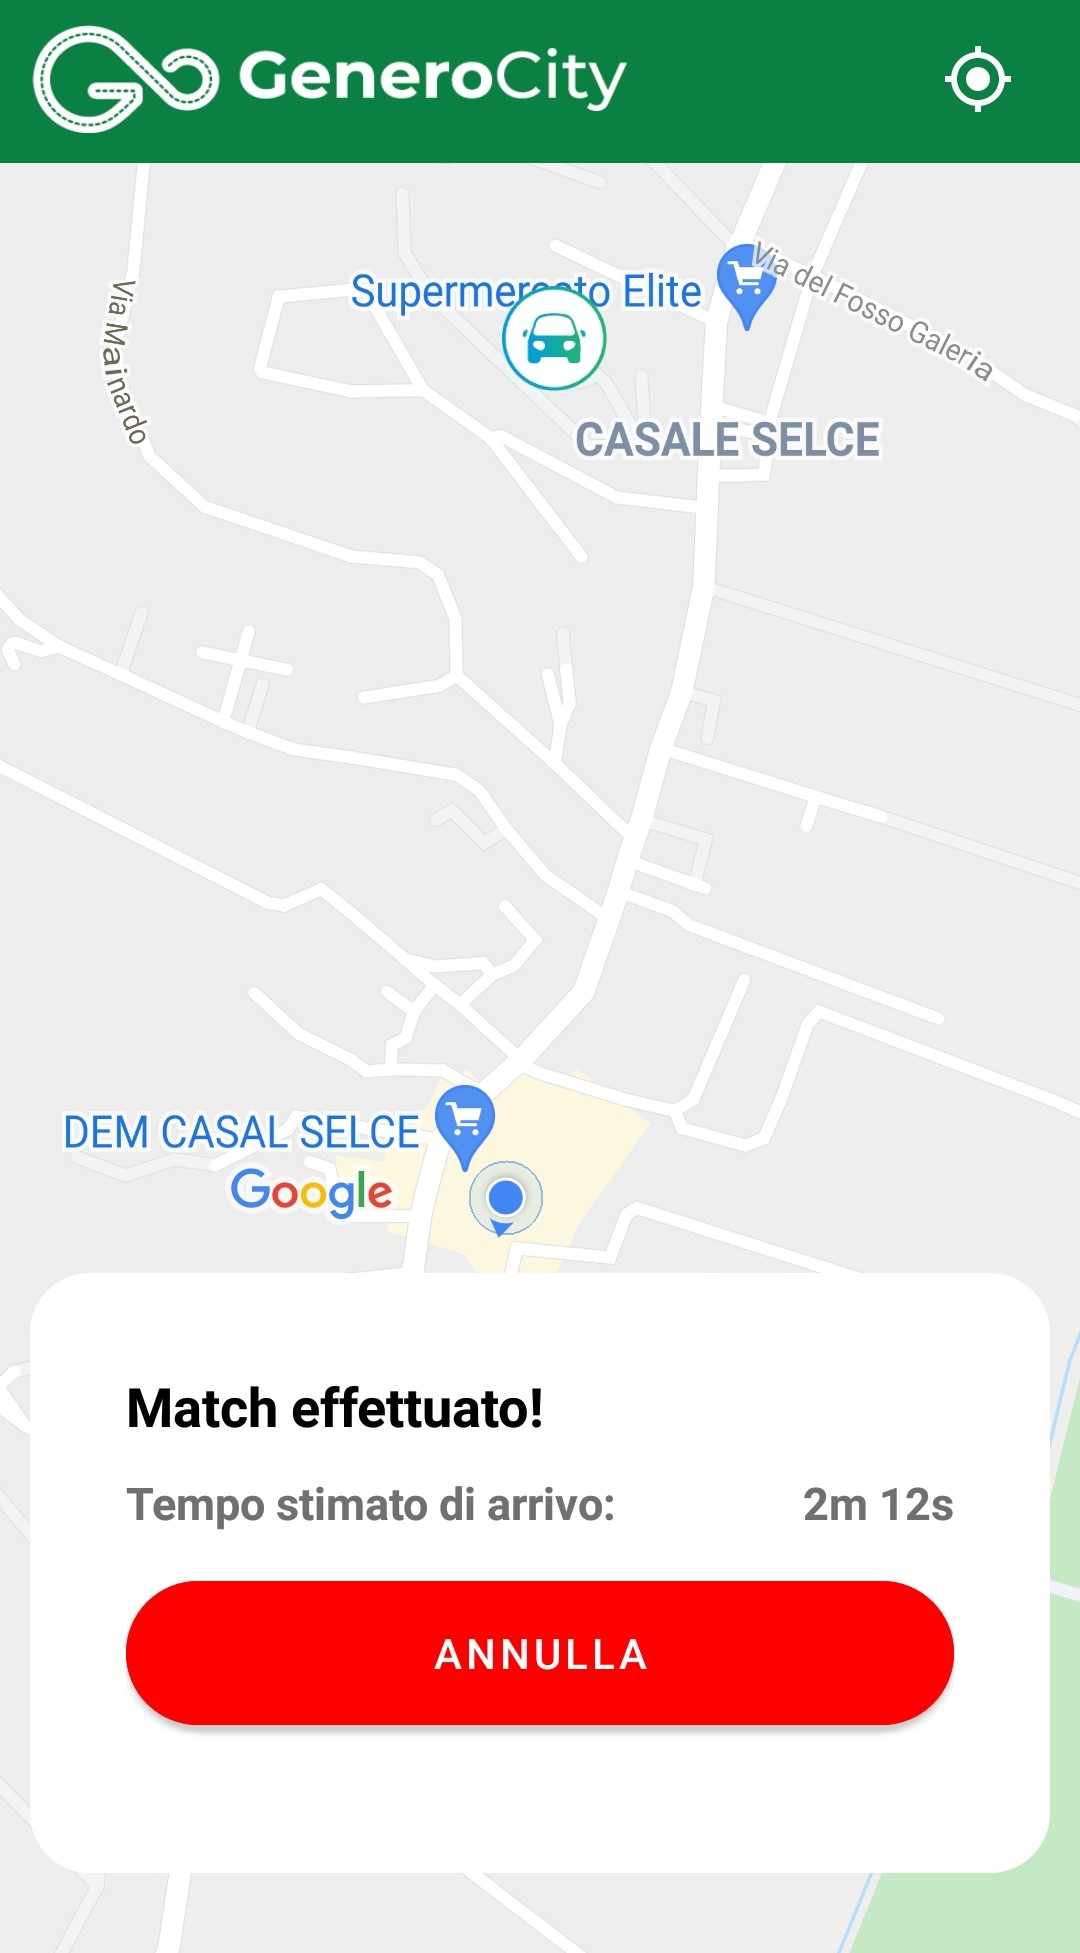
\includegraphics[width=6cm]{match_found_giver.jpg}
\caption{Interfaccia mostrata al Giver quando ha trovato un
Taker compatibile.}
\end{figure}


Per quanto riguarda il \texttt{Fragment} mostrato al Giver, sono presenti tre elementi:

\begin{itemize}
    \item Una \emph{label} che indica che un match è stato effettuato, e quindi che è presente un Taker compatibile a cui cedere il posto;
    \item Una \emph{label} che indica il tempo stimato circa l'incontro tra i due utenti;
    \item Un bottone con dicitura ``Annulla'' che permette di annullare il match in corso.
\end{itemize}
Nella mappa è presente il \textit{marker} che rappresenta la posizione, aggiornata in tempo reale, del Taker.

\hypertarget{aggiornamento-della-posizione-del-taker}{%
\subsubsection{Aggiornamento della posizione del taker}\label{aggiornamento-della-posizione-del-taker}}

Quando il Taker comincerà a guidare dirigendosi verso il
Giver, quest'ultimo vedrà sull'interfaccia il \emph{marker} che rappresenta la posizione del Taker muoversi in tempo reale.

Il risultato viene raggiunto nella seguente maniera:

\begin{enumerate}      
    \item Siano T e G rispettivamente il Taker ed il Giver all'interno di un match in stato Running;      
    \item Il client di T effettua, ogni \texttt{5000ms}, una chiamata alle API con endpoint \texttt{"/car/\{cid\}/position"} dove \texttt{\{cid\}} è il codice univoco dell'auto con cui il Taker vuole parcheggiare. La chiamata alle API ha un metodo \texttt{HTTP POST}, e richiede nel \texttt{body} un oggetto \texttt{json} con le informazioni relative alla posizione da inviare, che verranno documentate in dettaglio nella \autoref{invio-periodico-posizione-taker}.      
    \item Il server, alla ricezione di tale chiamata API, invia una notifica push al client del Giver, del tipo: 
        \begin{verbatim}  
        {x-gc-category:TAKERPOSITION, lat:42.2412, lon:12.4253, eta:2674}  
        \end{verbatim}      
    \item Il client di G, alla ricezione di ogni notifica push, estrae la nuova posizione di T ed aggiorna il rispettivo marker sulla mappa tramite un'animazione della durata di \texttt{5000ms}. 
\end{enumerate}

\hypertarget{tempo-previsto-per-larrivo-del-taker}{%
\subsubsection{Tempo previsto per l'incontro dei due utenti}\label{tempo-previsto-per-larrivo-del-taker}}

Su entrambe le interfacce viene mostrata l'informazione relativa al tempo rimanente stimato prima che i due utenti si incontrino.

Il Taker, immediatamente prima di effettuare una chiamata alle API per comunicare la posizione aggiornata al server, come visto nel paragrafo precedente, effettua una chiamata alle \emph{DistanceMatrix} Google APIs, all'url
\begin{verbatim}
    https://maps.googleapis.com/maps/api/distancematrix/json
\end{verbatim}
in cui vengono inseriti, come \textit{query parameters} i seguenti valori:
\begin{itemize}
    \item \texttt{origins}: le coordinate del punto d'origine, ovvero l'attuale posizione del Taker;
    \item \texttt{destinations}: le coordinate del punto destinazione, ovvero la posizione del Giver;
    \item \texttt{departure-time}: l'istante di partenza, impostato sempre su \texttt{now};
    \item \texttt{key}: la chiave per poter utilizzare le API.
\end{itemize}

Nell'oggetto json che il server manderà nel \texttt{body} della risposta alla chiamata API, sono presenti tre valori:
\begin{enumerate}
    \item Un valore che indica la distanza percorribile su strada, in metri, tra i due punti;
    \item Un valore che indica la durata del viaggio, in secondi, senza considerare il traffico;
    \item Un valore che indica la durata del viaggio, in secondi, considerando il traffico.
\end{enumerate}

Viene preso in considerazione solo il terzo valore che, una volta ottenuto, viene mostrato sull'interfaccia del Taker. Quando il Taker, immediatamente dopo, effettua la chiamata per aggiornate la posizione (\autoref{aggiornamento-della-posizione-del-taker}), inserisce tale valore nel campo \texttt{eta} all'interno del \texttt{body} della richiesta. 

Il Giver, alla ricezione della notifica vista in \autoref{aggiornamento-della-posizione-del-taker}, formatta il valore e lo inserisce nella sua interfaccia. 

\hypertarget{annullamento-di-un-match}{%
\subsection{Annullamento di un match}\label{annullamento-di-un-match}}

Un match, che sia in fase di ricerca o in corso, può essere annullato dalla parte di entrambi gli utenti coinvolti, mediante la pressione del bottone ``Annulla''.

\begin{figure}[H]
\centering
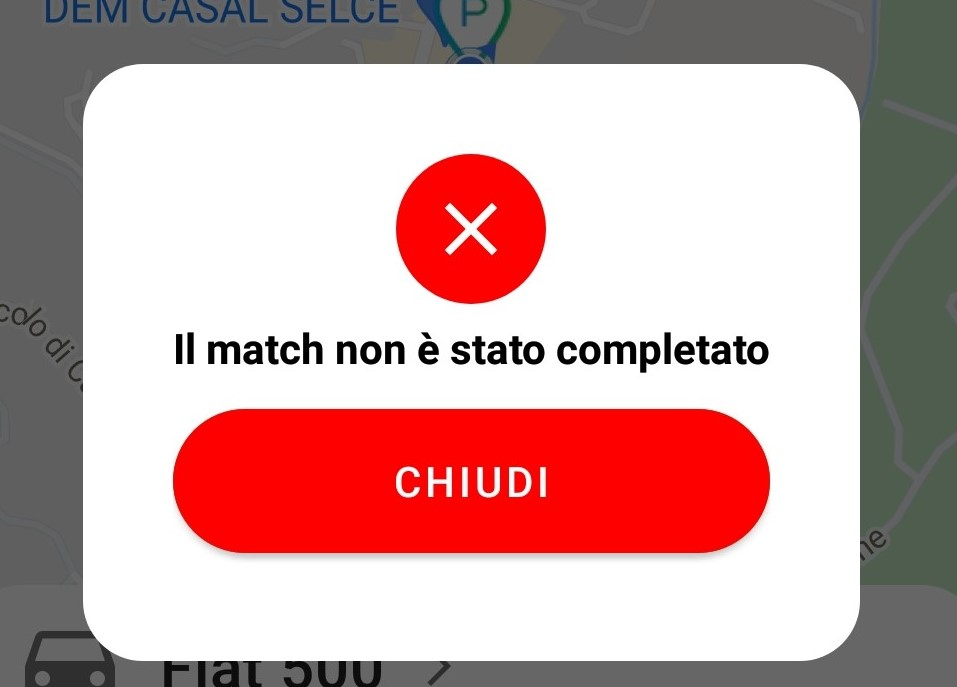
\includegraphics[width=6cm]{Dialog_match_non_completato.jpg}
\caption{Messaggio mostrato in caso il match non sia andato a buon
\label{Dialog_match_non_completato} fine.}
\end{figure}

\hypertarget{annullamento-di-un-match-in-fase-di-ricerca}{%
\subsubsection{Annullamento di un match in fase di ricerca}\label{annullamento-di-un-match-in-fase-di-ricerca}}

In caso di annullamento di un match in fase di ricerca, l'utente viene riportato alla schermata iniziale e viene mostrato una
\texttt{DialogWindow} (\autoref{Dialog_match_non_completato}) che comunica all'utente il corretto annullamento del match.

\hypertarget{annullamento-di-un-match-in-corso}{%
\subsubsection{Annullamento di un match in corso}\label{annullamento-di-un-match-in-corso}}

Visto che un match in corso comprende due utenti, l'annullamento da parte di un utente implica che il match venga annullato anche per il secondo utente.

Durante tutta la vita del frammento \texttt{MatchFoundFragment}, ovvero durante tutto il tempo in cui gli utenti sono all'interno di un match, un frammento di codice viene eseguito ogni 2 secondi, il cui scopo è quello di controllare se l'utente sia ancora in un match o meno. Questo avviene mediante una chiamata alle API.

Il flow dell'applicazione è quindi il seguente:

\begin{enumerate}
    \item Siano T e G rispettivamente un Taker ed un Giver all'interno di un match
    \item T annulla il match premendo sul pulsante ``Annulla'';
    \item T viene riportato alla pagina principale e gli viene mostrata la \emph{\texttt{DialogWindow}} che mostra i corretto annullamento del match (\autoref{Dialog_match_non_completato});
    \item Al più 2 secondi dopo dall'annullamento del match da parte di T, il codice che controlla lo stato del match riconosce che l'utente G non è più all'interno di un match;
    \item G viene riportato alla pagina principale e gli viene mostrata la medesima schermata di corretto annullamento del match.
\end{enumerate}

\hypertarget{completamento-di-un-match}{%
\subsection{Completamento di un match}\label{completamento-di-un-match}}

Un match può essere completato solamente se è in corso, e tale azione può essere effettuata solamente dal Taker, mediante la pressione del pulsante ``Completa'' nel \texttt{MatchFoundFragment}.

Il flow dell'applicazione è il seguente:

\begin{enumerate}

    \item Siano T e G rispettivamente un Taker ed un Giver all'interno di un match;
    \item T completa il match premendo sul pulsante ``Completa''';
    \item T viene riportato alla pagina principale e gli viene mostrata la \emph{\texttt{DialogWindow}} che mostra il corretto completamento del match (\autoref{Dialogo_match_completato});
    \item Al più 2 secondi dopo dall'annullamento del match da parte di T, il codice che controlla lo stato del match riconosce che il match che comprende G è stato completato;
    \item G viene riportato alla pagina principale e gli viene mostrata la \emph{\texttt{DialogWindow}} che mostra il corretto completamento del match (\autoref{Dialogo_match_completato};
\end{enumerate}

\begin{figure}[H]
\centering
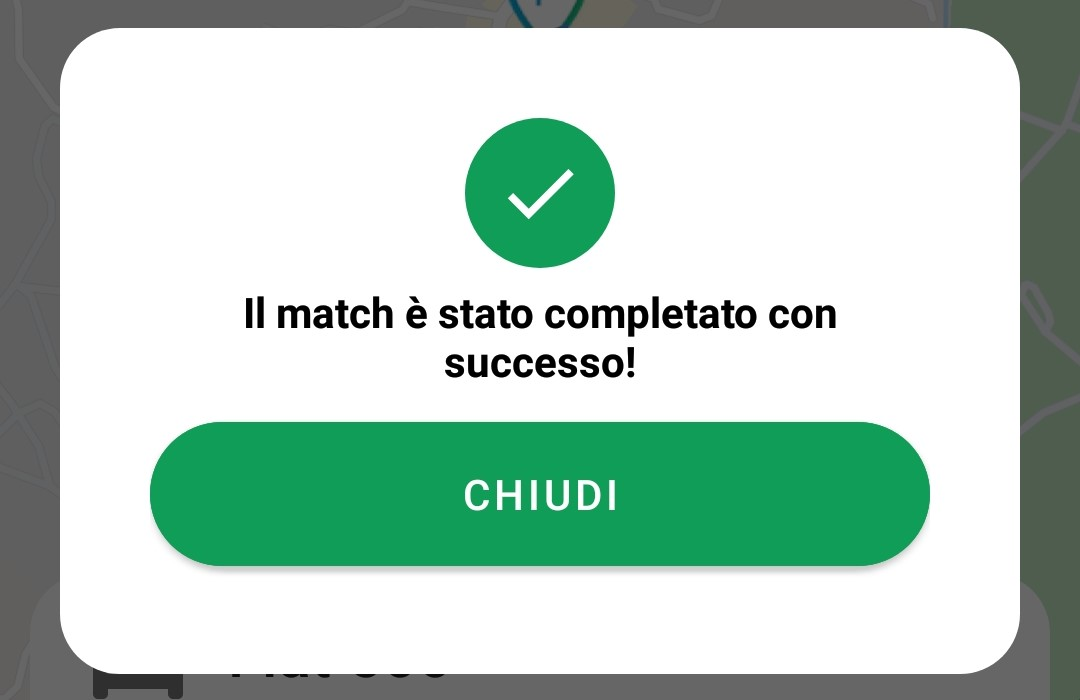
\includegraphics[width=6cm]{Dialogo_match_completato.jpg}
\caption{Messaggio mostrato in caso il match sia stato completato con successo.}
\label{Dialogo_match_completato}
\end{figure}

\hypertarget{modificare-posizione-parcheggio}{%
\section{Modifica posizione parcheggio}\label{modificare-posizione-parcheggio}}

Nello stato dell'applicazione prima dell'implementazione della modifica di cui si andrà a parlare, per l'utente non era possibile modificare la posizione di un parcheggio effettuato precedentemente.

\hypertarget{prima-iterazione}{%
\subsection{Prima iterazione}\label{prima-iterazione}}

\hypertarget{info-window}{%
\subsubsection{Info Window}\label{info-window}}

La \texttt{InfoWindow} è l'elemento che appare quando si clicca sopra un
\emph{marker} all'interno di una mappa. Tale elemento può essere personalizzato a piacere in maniera da contenere le informazioni che possono risultare più utili all'utente. Viene quindi aggiunta una funzionalità che permette all'utente di modificare la posizione del parcheggio in cui l'auto è attualmente parcheggiata. 

\begin{figure}[H]
\centering
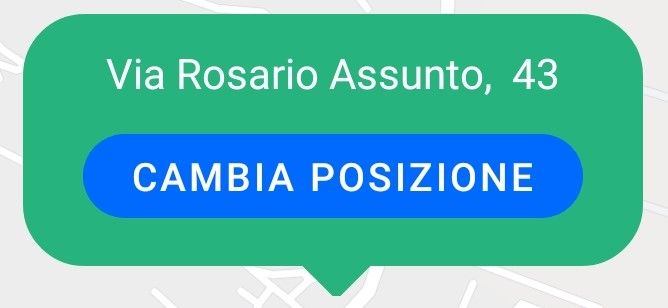
\includegraphics[width=6cm]{CustomInfoWindowCut.jpg}
\caption{La \texttt{InfoWindow} relativa al marker del parcheggio}
\label{info-window}
\end{figure}

In tale elemento sono presenti tre elementi:

\begin{itemize}
    \item L'indirizzo in cui è situato il \emph{marker};
    \item La distanza che separa la posizione del marker dalla posizione attuale dell'utente;
    \item Un pulsante che permette di modificare la posizione del \emph{marker};
\end{itemize}
\hypertarget{ui-per-la-modifica-del-parcheggio}{%
\subsubsection{UI per la modifica del parcheggio}\label{ui-per-la-modifica-del-parcheggio}}

\begin{figure}[H]
\centering
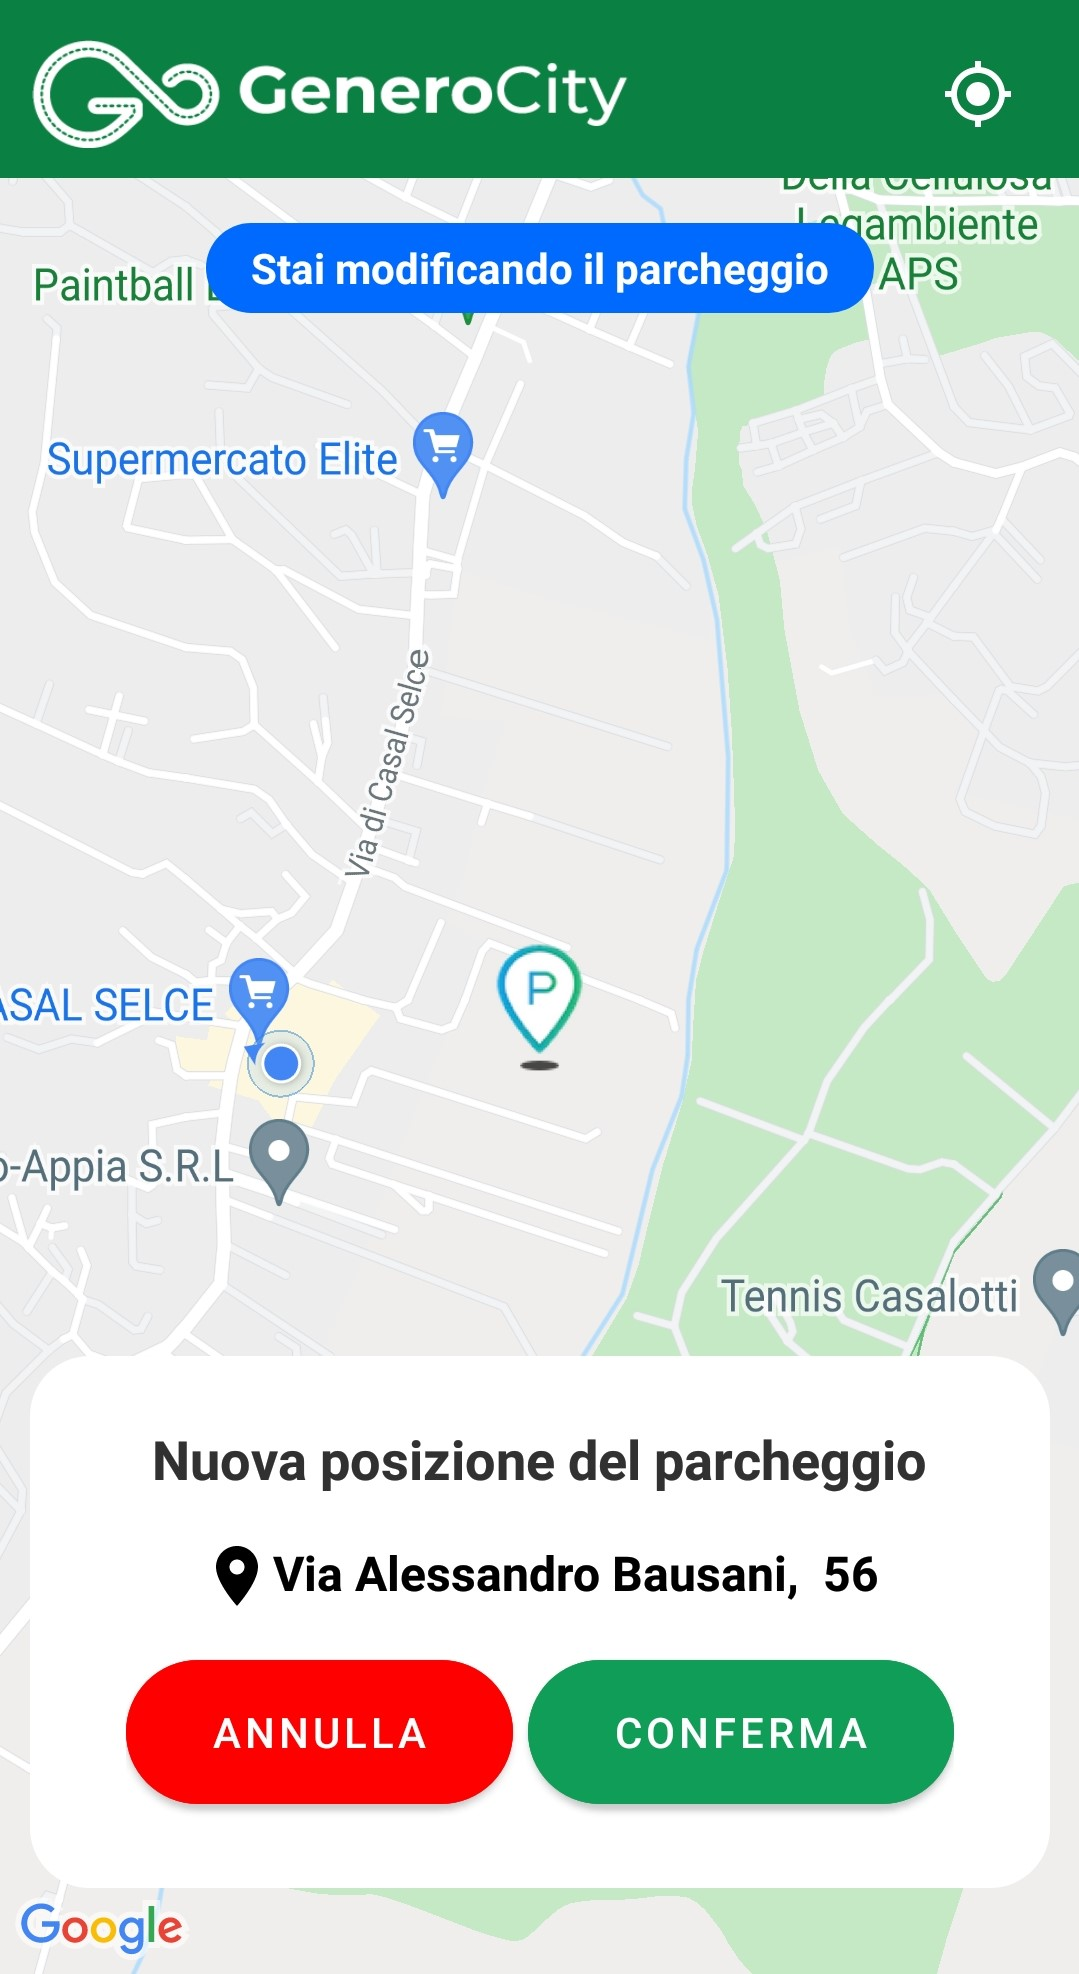
\includegraphics[width=6cm]{EditMode.jpg}
\caption{Prima iterazione della schermata per la modifica del parcheggio.}
\end{figure}

L'utente può scegliere la nuova posizione del parcheggio muovendo la mappa. Il \emph{marker} che segna la nuova posizione rimarrà sempre al centro dello schermo.

Si può accedere a tale schermata in due modi:

\begin{itemize}
    \item Tenendo premuto a lungo sulla mappa;
    \item Premendo sul bottone mostrato in \autoref{info-window} all'interno della \texttt{InfoWindow}.
\end{itemize}
La schermata presenta vari elementi:

\begin{itemize}
    \item Un \emph{fragment} in alto, sotto alla \emph{app bar}, che indica che l'utente si trova all'interno della schermata per la modifica del parcheggio;
    \item Una label che indica la nuova posizione del parcheggio, ovvero la conversione da coordinate ad indirizzo del punto sulla mappa in cui è situato il \emph{marker}. 
    \item Un pulsante ``Annulla'' che consente di annullare la modifica del parcheggio. Una volta premuto tale pulsante l'utente verrà reindirizzato alla pagina principale ed il parcheggio non sarà modificato;
    \item Un pulsante ``Conferma'' che consente di completare la modifica del parcheggio. Una volta premuto tale pulsante l'utente verrà reindirizzato alla pagina principale, e la posizione del parcheggio sarà modificata con la nuova posizione scelta dall'utente.
\end{itemize}
\hypertarget{icona-del-marker}{%
\subsubsection{Icona del marker}\label{icona-del-marker}}

\begin{figure}[H]
\centering

\includegraphics[width=2cm]{images/park_pin.png}
\caption{Marker di un parcheggio effettuato.}
\label{park-pin}
\end{figure}

La \autoref{park-pin} mostra il marker che indica la posizione di un parcheggio sulla mappa.

\begin{figure}[H]
\centering

\includegraphics[width=1.7cm]{park_pin_shadow.png}
\caption{Marker della potenziale nuova posizione del parcheggio.}
\label{park-pin-shadow}
\end{figure}

La \autoref{park-pin-shadow} mostra l'icona presente al centro dello schermo quando l'utente si trova nella \emph{activity} per modificare la posizione del parcheggio. In questo caso l'icona, molto simile a quella in \autoref{park-pin}, presenta un'ombra sottostante in modo da far capire all'utente, mediante l'utilizzo di una metafora, che il marker non è ``fissato'' sulla mappa ma può essere spostato.

\hypertarget{test}{%
\subsubsection{Test}\label{test}}

Per verificare l'usabilità dell'interfaccia sono stati effettuati dei test con degli utenti.

Tali utenti sono stati inseriti in una situazione ipotetica, ed è stato chiesto loro di modificare la posizione del parcheggio nell'applicazione.

Gli utenti non sono riusciti a capire in che maniera raggiungere la schermata per modificare la posizione del parcheggio.

Una volta fatti entrare nella schermata desiderata, gli utenti sono riusciti a modificare il parcheggio, ma alcuni utenti hanno fatto difficoltà a trovare l'indirizzo comunicato.

\hypertarget{problemi-rilevati}{%
\subsubsection{Problemi rilevati}\label{problemi-rilevati}}

Dai test effettuati sono state rilevate le seguenti problematiche:

\begin{itemize}
    \item Il \emph{marker} del parcheggio non sembra cliccabile;
    \item La pressione lunga sulla mappa è un comando nascosto;
    \item Cercare la via spostandosi sulla mappa è utile per modifiche di distanze minori, ma è poco comodo in caso l'utente debba modificare il parcheggio in una posizione completamente differente.
\end{itemize}
\hypertarget{seconda-iterazione}{%
\subsection{Seconda iterazione}\label{seconda-iterazione}}

I primi due problemi individuati nella prima iterazione del prototipo sono stati risolti inserendo un \texttt{FloatingActionButton} nella pagina dei dettagli del parcheggio corrente. Visto che è possibile modificare solamente tale parcheggio, il \texttt{FloatingActionButton} non viene mostrato all'interno delle schermate di dettaglio dei parcheggi effettuati precedentemente.

\begin{figure}[H]
\centering
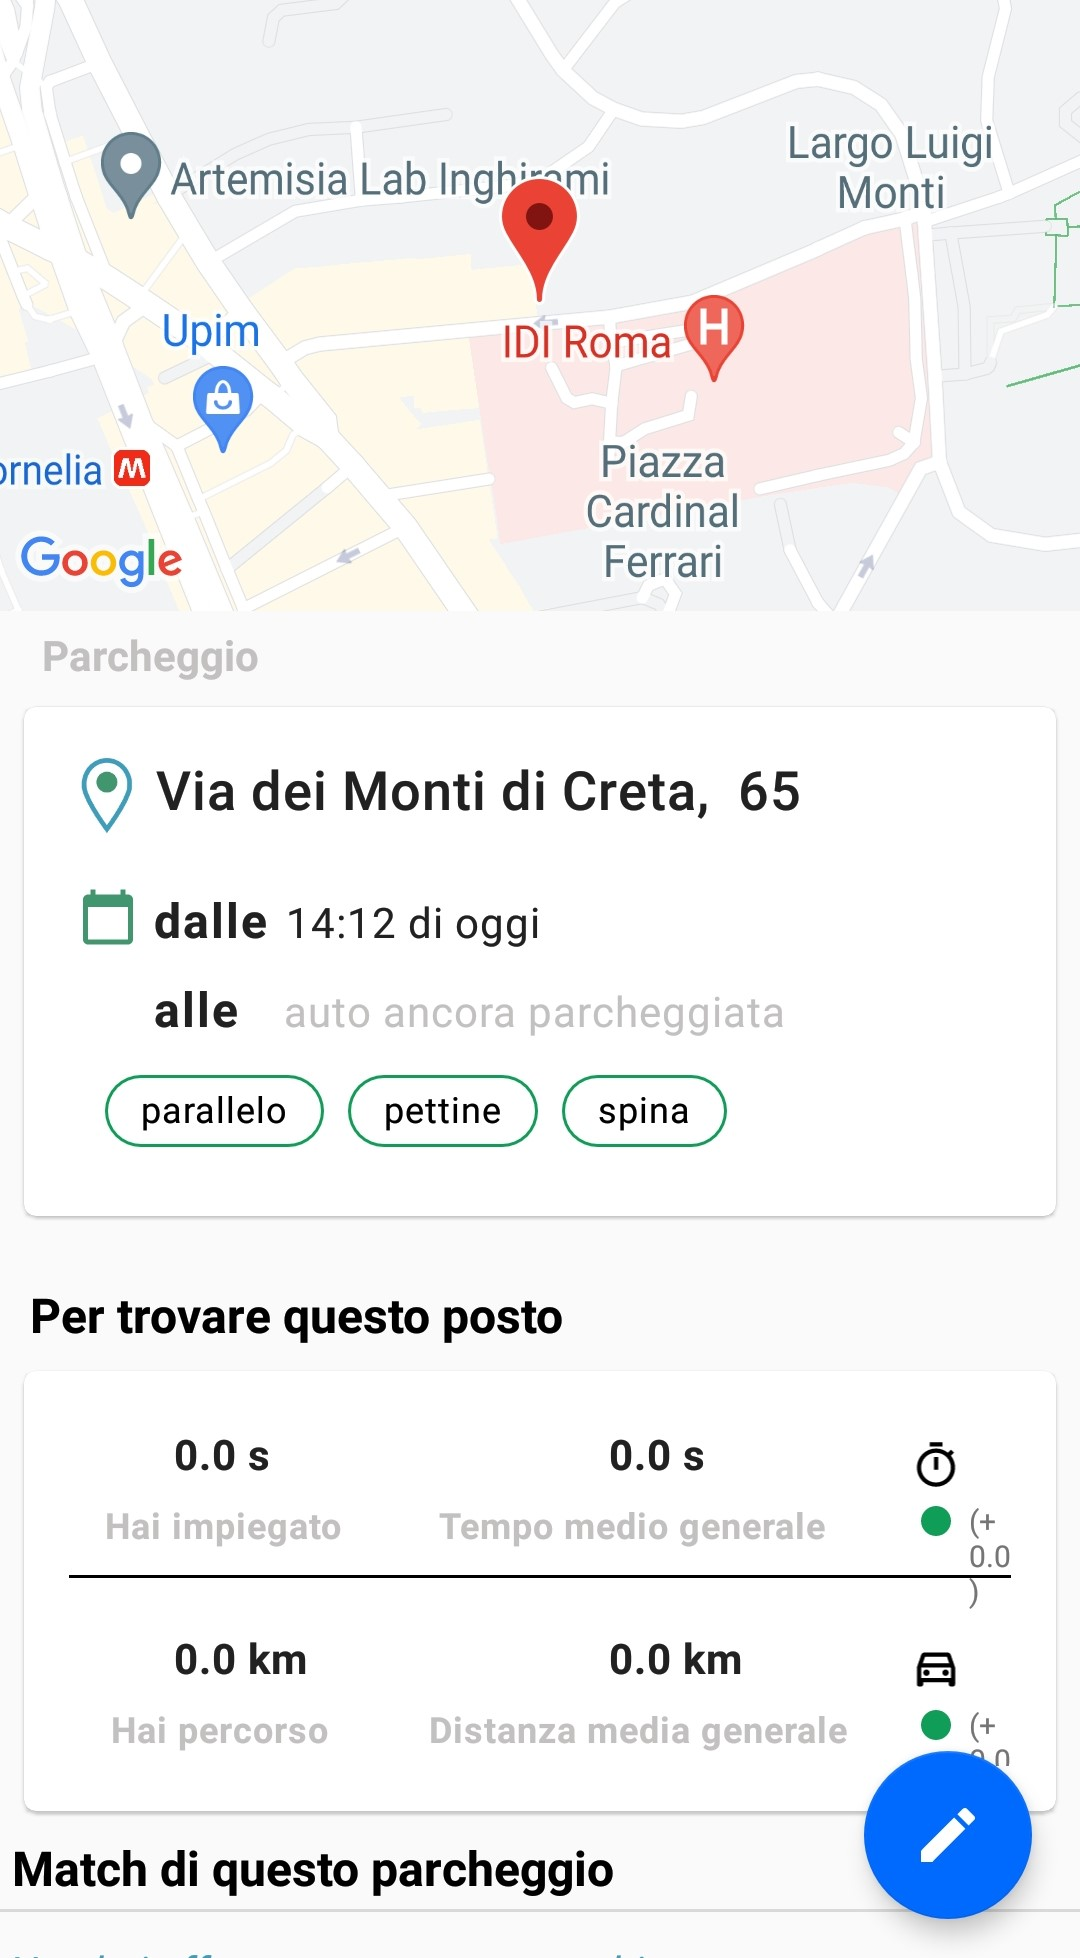
\includegraphics[width=6cm]{Floating_Action_Button.jpg}
\caption{Pagina dei dettagli di un parcheggio con
\texttt{FloatingActionButton}}
\end{figure}

È stata presa questa decisione in quanto, nei test effettuati, gli utenti navigavano nella pagina contenente i dettagli di un parcheggio cercando un modo per modificare l'indirizzo.

Il terzo problema è stato risolto rendendo modificabile l'indirizzo presente nel \texttt{ChangeParkPositionFragment}. In questa maniera l'utente è sempre al corrente del nuovo indirizzo del parcheggio, ma può cliccare su di esso per modificarlo tramite tastiera.

\begin{figure}[H]
\centering
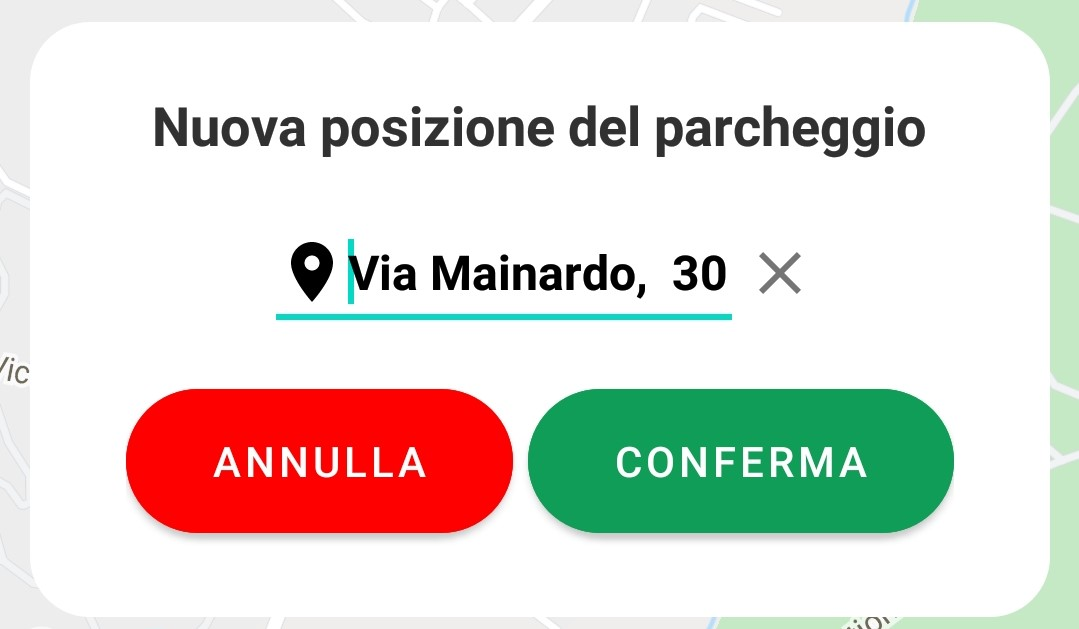
\includegraphics[width=6cm]{images/Editable_new_address.jpg}
\caption{\texttt{ChangeParkPositionFragment} con indirizzo modificabile}
\end{figure}

\hypertarget{test-1}{%
\subsubsection{Test}\label{test-1}}

Sono stati effettuati ulteriori test utilizzando la seconda iterazione dell'interfaccia e gli utenti sono riusciti a modificare il parcheggio utilizzando il \texttt{FloatingActionButton} nella pagina dei dettagli del parcheggio corrente.

Una volta entrati nella schermata per la modifica del parcheggio, gli utenti hanno spostato la mappa manualmente quando si chiedeva loro di modificare la posizione del parcheggio in una posizione molto vicina a quella attuale, mentre hanno utilizzato il campo di testo editabile quando è stato chiesto loro di modificare la posizione del parcheggio in una via più distante dalla posizione attuale, e quindi più difficile da trovare muovendo manualmente la mappa.

Non sono stati trovati ulteriori problemi di usabilità, e quindi l'interfaccia può essere considerata definitiva. 
